%iffalse
\documentclass[journal]{IEEEtran}
\usepackage[a5paper, margin=10mm]{geometry}
%\usepackage{lmodern} % Ensure lmodern is loaded for pdflatex
\usepackage{tfrupee} % Include tfrupee package


\setlength{\headheight}{1cm} % Set the height of the header box
\setlength{\headsep}{0mm}     % Set the distance between the header box and the top of the text


%\usepackage[a5paper, top=10mm, bottom=10mm, left=10mm, right=10mm]{geometry}

%
\setlength{\intextsep}{10pt} % Space between text and floats

\makeindex


\usepackage{cite}
\usepackage{amsmath,amssymb,amsfonts,amsthm}
\usepackage{algorithmic}
\usepackage{graphicx}
\usepackage{textcomp}
\usepackage{xcolor}
\usepackage{txfonts}
\usepackage{listings}
\usepackage{enumitem}
\usepackage{mathtools}
\usepackage{gensymb}
\usepackage{comment}
\usepackage[breaklinks=true]{hyperref}
\usepackage{tkz-euclide} 
\usepackage{listings}
\usepackage{multicol}
\usepackage{xparse}
\usepackage{gvv}
%\def\inputGnumericTable{}                                 
\usepackage[latin1]{inputenc}                                
\usepackage{color}                                            
\usepackage{array}                                            
\usepackage{longtable}                                       
\usepackage{calc}                                             
\usepackage{multirow}                                         
\usepackage{hhline}                                           
\usepackage{ifthen}  
\usepackage{wrapfig}
\usepackage{lscape}
\usepackage{tabularx}
\usepackage{array}
\usepackage{float}
\usepackage[justification=centering]{caption}


\newtheorem{theorem}{Theorem}[section]
\newtheorem{problem}{Problem}
\newtheorem{proposition}{Proposition}[section]
\newtheorem{lemma}{Lemma}[section]
\newtheorem{corollary}[theorem]{Corollary}
\newtheorem{example}{Example}[section]
\newtheorem{definition}[problem]{Definition}
\newcommand{\BEQA}{\begin{eqnarray}}
\newcommand{\EEQA}{\end{eqnarray}}

\theoremstyle{remark}


\begin{document}
\bibliographystyle{IEEEtran}
\onecolumn

\title{Naval Architecture and Marine Engineering}
\author{EE25BTECH11026-Harsha}
\maketitle

\renewcommand{\thefigure}{\theenumi}
\renewcommand{\thetable}{\theenumi}
\setcounter{secnumdepth}{0}
\subsection{\underline{\textbf{General Aptitude (G.A)}}}
\subsubsection{\underline{Q.1 \text{-} Q.5 Carry ONE mark Each}}
\setlength{\parskip}{1em}

\begin{enumerate}
\item Despite his initial hesitation, Rehman's \underline{\hspace{1cm}} to contribute to the success of
the project never wavered. Select the most appropriate option to complete the above sentence.
\begin{multicols}{4}
\begin{enumerate}
    \item ambivalence
    \item satisfaction
    \item resolve
    \item revolve
\end{enumerate}
\end{multicols}
\end{enumerate}

\begin{enumerate}[itemsep=1em]
\setcounter{enumi}{1}
\item Bird : Nest :: Bee : \underline{\hspace{1cm}}\\
\\
Select the correct option to complete the analogy.
\begin{multicols}{4}
\begin{enumerate}
    \item Kennel
    \item Hammock
    \item Hive
    \item Lair
\end{enumerate}
\end{multicols}
\end{enumerate}

\begin{enumerate}[itemsep=1em]
\setcounter{enumi}{2}
\item If $Pe^x=Qe^{-x}$ for all real values of $x$, which one of the following statements is true?
\begin{multicols}{4}
\begin{enumerate}
    \item $P=Q=0$
    \item $P=Q=1$
    \item $P=1\,;Q=1$
    \item $\frac{P}{Q}=0$
\end{enumerate}
\end{multicols}
\end{enumerate}

\begin{enumerate}[itemsep=1em]
\setcounter{enumi}{3}
\item The paper as shown in the figure is folded to make a cube where each square corresponds to a particular face of the cube. Which one of the following options correctly represents the cube?\\
\\
Note: The figures shown are representative.
\begin{figure}[H]
    \centering
    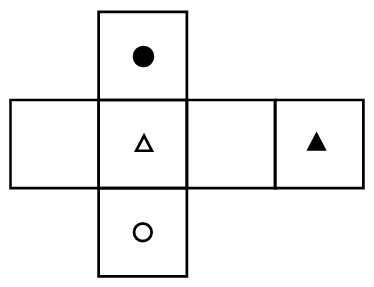
\includegraphics[width=0.2\columnwidth]{figs/fig-1.jpeg}
    \caption*{Fig-1}
    \label{fig:1}
\end{figure}
\newpage
\vspace*{0.25cm}
\begin{multicols}{4}
\begin{enumerate}
    \item \begin{minipage}[t]{0.2\textwidth}
    \vspace{0pt}
        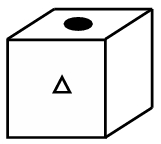
\includegraphics[width=\columnwidth]{figs/fig-2.jpeg}
        \label{fig:2}
    \end{minipage}
    \item \begin{minipage}[t]{0.2\textwidth}
    \vspace{0pt}
        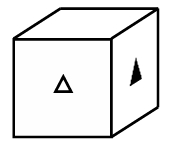
\includegraphics[width=\columnwidth]{figs/fig-3.jpeg}
        \label{fig:3}
    \end{minipage}
    \item \begin{minipage}[t]{0.2\textwidth}
    \vspace{0pt}
        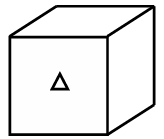
\includegraphics[width=\columnwidth]{figs/fig-4.jpeg}
        \label{fig:4}
    \end{minipage}
    \item \begin{minipage}[t]{0.2\textwidth}
    \vspace{0pt}
        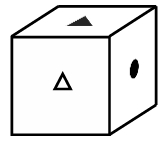
\includegraphics[width=\columnwidth]{figs/fig-5.jpeg}
    \label{fig:5}
    \end{minipage}
\end{enumerate}
\end{multicols}
\end{enumerate}

\begin{enumerate}[itemsep=1em]
\setcounter{enumi}{4}
\item Let $p_1$ and $p_2$ denote two arbitrary prime numbers. Which one of the following statements is correct for all values of $p_1$ and $p_2$? 
\begin{enumerate}[leftmargin=2.5em, labelsep=0.5em, itemsep=0.5em]
    \item $p_1 + p_2$ is not a prime number. 
    \item $p_1p_2$ is not a prime number.
    \item $p_1+p_2+1$ is a prime number.
    \item $p_1p_2+1$ is a prime number.
\end{enumerate}
\end{enumerate}

\subsubsection{\underline{Q.6 \text{-} Q.10 Carry TWO marks Each}}
\setlength{\parskip}{1em}

\begin{enumerate}[itemsep=1em]
\setcounter{enumi}{5}
\item Based only on the conversation below, identify the logically correct inference: \\
\\
"Even if I had known that you were in the hospital, I would not have gone there to see you", Ramya told Josephine. 

\begin{enumerate}[leftmargin=2.5em, labelsep=0.5em, itemsep=0.5em]
   \item Ramya knew that Josephine was in the hospital. 
   \item Ramya did not know that Josephine was in the hospital. 
   \item Ramya and Josephine were once close friends; but now, they are not. 
   \item Josephine was in the hospital due to an injury to her leg. 
\end{enumerate}
\end{enumerate}

\begin{enumerate}[itemsep=1em]
\setcounter{enumi}{6}
\item If IMAGE and FIELD are coded as FHBNJ and EMFJG respectively then, which one among the given options is the most appropriate code for BEACH ? 

\begin{multicols}{4}
\begin{enumerate}
    \item CEADP
    \item IDBFC
    \item JGIBC
    \item IBCEC
\end{enumerate}
\end{multicols}
\end{enumerate}

\newpage
\vspace*{0.25cm}

\begin{enumerate}[itemsep=1em]
\setcounter{enumi}{7}
\item Which one of the following options is correct for the given data in the table?  
\begin{figure}[H]
    \centering
    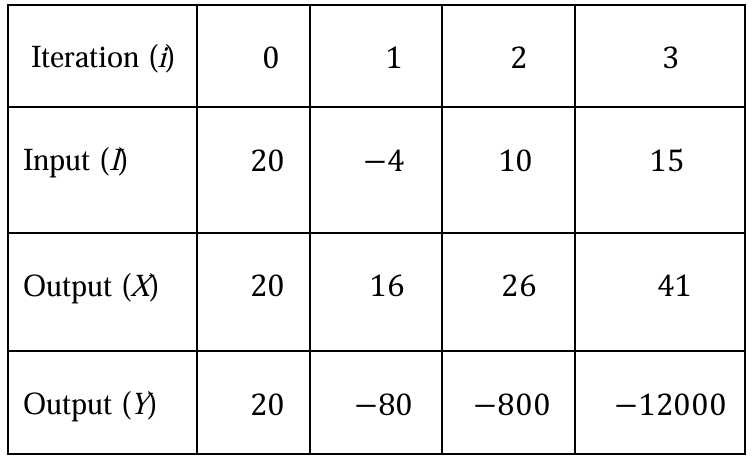
\includegraphics[width=0.4\columnwidth]{figs/fig-6.jpeg}
    \caption*{Fig-6:Data table}
    \label{fig:6}
\end{figure}
\begin{enumerate}[leftmargin=2.5em, labelsep=0.5em, itemsep=0.5em]
    \item $X(i)=X(i-1)+I(i);\;\;Y(i)=Y(i-1)I(i);\;\;i>0$
    \item $X(i)=X(i-1)I(i);\;\;Y(i)=Y(i-1)+I(i);\;i>0$
    \item $X(i)=X(i-1)I(i);\;\;Y(i)=Y(i-1)I(i);\;i>0$
    \item $X(i)=X(i-1)+I(i);\;\;Y(i)=Y(i-1)I(i-1);\;i>0$
\end{enumerate}
\end{enumerate}

\begin{enumerate}[itemsep=1em]
\setcounter{enumi}{8}
\item In the given figure, PQRS is a square of side 2 cm and PLMN is a rectangle. The corner L of the rectangle is on the side QR. Side MN of the rectangle passes through the corner S of the square. What is the area (in $cm^2$) of the rectangle PLMN?\\
\\
Note: The figure shown is representative. 
\begin{figure}[H]
    \centering
    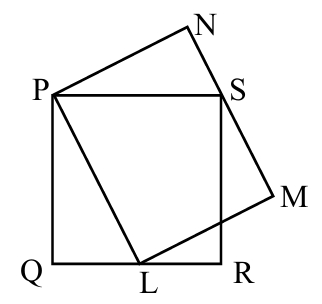
\includegraphics[width=0.4\columnwidth]{figs/fig-7.jpeg}
    \caption*{Fig-7:Square PQRS and Rectangle PLMN}
    \label{fig:7}
\end{figure}
\begin{multicols}{4}
\begin{enumerate}
    \item $2\sqrt{2}$
    \item $2$
    \item 8
    \item 4
\end{enumerate}
\end{multicols}
\end{enumerate}
\newpage
\vspace*{0.25cm}
\begin{enumerate}[itemsep=1em]
\setcounter{enumi}{9}
\item The diagram below shows a river system consisting of 7 segments, marked P, Q, R, S, T, U, and V. It splits the land into 5 zones, marked Z1, Z2, Z3, Z4, and Z5. We need to connect these zones using the least number of bridges. Out of the following options, which one is correct? \\
\\
Note: The figure shown is representative. 
\begin{figure}[H]
    \centering
    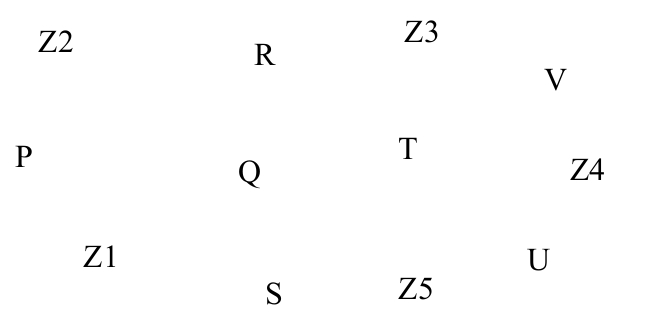
\includegraphics[width=0.4\columnwidth]{figs/fig-8.jpeg}
    \caption*{Fig-8:River system}
    \label{fig:8}
\end{figure}
\begin{enumerate}[leftmargin=2.5em, labelsep=0.5em, itemsep=0.5em]
    \item Bridges on P, Q, and T 
    \item Bridges on P, Q, S, and T 
    \item Bridges on Q, R, T, and V 
    \item Bridges on P, Q, S, U, and V 
\end{enumerate}
\end{enumerate}

\subsubsection{\underline{Q.11 \text{-} Q.35 Carry TWO marks Each}}
\setlength{\parskip}{1em}

\begin{enumerate}[itemsep=1em]
\setcounter{enumi}{10}
    \item The value of $\lim\limits_{t \to 1}\frac{ln\,t}{t^2-1}$ is \underline{\hspace{0.5cm}}.

\begin{multicols}{4}
\begin{enumerate}
    \item $\frac{1}{2}$
    \item 0
    \item 1
    \item $\infty$
\end{enumerate}
\end{multicols}
\end{enumerate}

\begin{enumerate}[itemsep=1em]
\setcounter{enumi}{11}
\item The Fourier series expansion of $f(x)=\sin^2{x}$ in the interval $(-\pi,\pi)$ is \underline{\hspace{1cm}}. 

\begin{enumerate}[leftmargin=2.5em, labelsep=0.5em, itemsep=0.5em]
    \item $f(x)=\frac{1}{2}-\frac{1}{2}\cos{2x}$
    \item $f(x)=\sum_{n=1}^{\infty}\,(-1)^{n-1}\frac{\cos{nx}}{n^2}$
    \item $f(x)=2\sum_{n=1}^{\infty}\,\frac{\sin{2nx}}{n}$
    \item $f(x)=\frac{1}{2}-\frac{4}{\pi^2}\sum_{n=1}^{\infty}\frac{\cos{(2n-1)\pi x}}{(2n-1)^2}$
\end{enumerate}
\end{enumerate}

\newpage
\vspace*{0.25cm}

\begin{enumerate}[itemsep=1em]
\setcounter{enumi}{12}
\item For all real values of x and y, the partial differential equation in terms of $\psi(x,y)$ given by $\frac{\partial^2\psi}{\partial x^2}+2\frac{\partial^2\psi}{\partial x \partial y }-3\frac{\partial^2\psi}{\partial y^2}=0$ is \underline{\hspace{1cm}}.
\begin{enumerate}[leftmargin=2.5em, labelsep=0.5em, itemsep=0.5em]
    \item hyperbolic 
    \item parabolic  
    \item elliptic 
    \item elliptic within the region, $x^2-y<0$
\end{enumerate}
\end{enumerate}

\begin{enumerate}[itemsep=1em]
\setcounter{enumi}{13}
\item The sum of the static pressure and dynamic pressure at a point in a fluid flow is called the \underline{\hspace{1cm}}. 
\begin{enumerate}[leftmargin=2.5em, labelsep=0.5em, itemsep=0.5em]
    \item kinematic pressure
    \item vacuum pressure
    \item stagnation pressure
    \item kinetic pressure
    
\end{enumerate}    
\end{enumerate}

\begin{enumerate}[itemsep=1em]
\setcounter{enumi}{14}
\item Identify the range of Reynolds number (Re) for a creeping flow. 

\begin{enumerate}[leftmargin=2.5em, labelsep=0.5em, itemsep=0.5em]
    \item $2000 < Re < 20000$ 
    \item $1000 < Re < 2000$ 
    \item $10 < Re < 100$ 
    \item $Re << 1$ 
\end{enumerate}   
\end{enumerate}

\begin{enumerate}[itemsep=1em]
\setcounter{enumi}{15}
\item The ratio of the magnitudes of vorticity to rate of rotation in a fluid flow is \underline{\hspace{1cm}}.
\begin{multicols}{4}
\begin{enumerate}
    \item 2
    \item 3
    \item $\frac{1}{2}$
    \item 1
\end{enumerate}
\end{multicols}
\end{enumerate}

\begin{enumerate}[itemsep=1em]
\setcounter{enumi}{16}
\item In a laminar boundary layer, the ratio of boundary layer thickness $(\delta)$ to the corresponding displacement thickness $(\delta^*)$ lies between \underline{\hspace{1cm}}. 
\begin{multicols}{4}
\begin{enumerate}
    \item 1.5 and 2.4
    \item 2.5 and 3.4
    \item 3.5 and 4.4
    \item 4.5 and 5.4
\end{enumerate}
\end{multicols}
\end{enumerate}

\begin{enumerate}[itemsep=1em]
\setcounter{enumi}{17}
\item  For marine engine shafts subjected to high radial and axial thrust loads, which one of the following types of bearings is the most suitable? 
\begin{enumerate}[leftmargin=2.5em, labelsep=0.5em, itemsep=0.5em]
    \item Deep groove ball
    \item Sealed ball
    \item Tapered ball
    \item Needle
\end{enumerate}

\end{enumerate}

\newpage
\vspace*{0.25cm}

\begin{enumerate}[itemsep=1em]
\setcounter{enumi}{18}
\item Which one of the following wave energy spectra is formulated for two peaks? 
\begin{enumerate}[leftmargin=2.5em, labelsep=0.5em, itemsep=0.5em]
    \item Pierson-Moskowitz spectrum 
    \item JONSWAP spectrum
    \item Ochi-Hubble spectrum
    \item Neumann spectrum
\end{enumerate}
\end{enumerate}

\begin{enumerate}[itemsep=1em]
\setcounter{enumi}{19}
\item According to linear water wave theory, at a point on the free surface of a regular wave, the phase difference between the free surface elevation and the horizontal water particle acceleration is \underline{\hspace{1cm}}. 
\begin{multicols}{4}
\begin{enumerate}
    \item $0\degree$
    \item $45\degree$
    \item $90\degree$
    \item $135\degree$
\end{enumerate}
\end{multicols}
\end{enumerate}

\begin{enumerate}[itemsep=1em]
\setcounter{enumi}{20}
\item The dynamic response amplitude $|H(\omega)|$ of a single degree of freedom system subjected to support motion is given by the following expression.
\[
|H(\omega)|=\sqrt{\frac{1+4\zeta^2(\frac{\omega}{\omega_n})^2}{[1-(\frac{\omega}{\omega_n})^2]^2+4\zeta^2(\frac{\omega}{\omega_n})^2}}
\]
$|H(\omega)|$ increases with an increase in damping ratio $(\zeta)$ if the excitation frequency $(\omega)$ is \underline{\hspace{1cm}} the natural frequency $(\omega_n)$ of the system.
\begin{multicols}{4}
\begin{enumerate}
    \item equal to
    \item 0.75 times
    \item $\frac{\sqrt{3}}{2}$ times
    \item greater than $\sqrt{2}$ times
\end{enumerate}
\end{multicols}
\end{enumerate}

\begin{enumerate}[itemsep=1em]
\setcounter{enumi}{21}
\item In the stress-strain curve of mild steel, plastic deformation starts at the \underline{\hspace{2cm}}.
\begin{enumerate}[leftmargin=2.5em, labelsep=0.5em, itemsep=0.5em]
    \item proportional limit
    \item elastic limit
    \item upper yield point
    \item lower yield point
\end{enumerate}
\end{enumerate}

\begin{enumerate}[itemsep=1em]
\setcounter{enumi}{22}
\item In ships, a flash evaporator is used to obtain \underline{\hspace{1cm}}.
\begin{enumerate}[leftmargin=2.5em, labelsep=0.5em, itemsep=0.5em]
    \item distilled water
    \item low viscosity lubricating oil
    \item high-temperature heavy oil
    \item air for space heating
\end{enumerate}
\end{enumerate}

\newpage
\vspace*{0.25cm}

\begin{enumerate}[itemsep=1em]
\setcounter{enumi}{23}
\item Which one of the following is the most common type of gear assembly used for coupling steam turbine and propeller shafts?
\begin{multicols}{4}
\begin{enumerate}
    \item Spur
    \item Single helical
    \item Double Helical
    \item Worm
\end{enumerate}
\end{multicols}
\end{enumerate}

\begin{enumerate}[itemsep=1em]
\setcounter{enumi}{24}
\item A ship of 5000 tonne displacement has two empty rectangular double bottom tanks with dimensions:\\
Tank A: length 12 m, width 16 m, and height 2 m\\
Tank B: length 16 m, width 12 m, and height 2 m\\
The length of each tank is oriented along the length of the ship. It is required to ballast the ship with 192 $m^3$ of seawater of density 1025 $kg/m^3$. Which one of the following scenarios will minimize the free surface effect?
\begin{enumerate}[leftmargin=2.5em, labelsep=0.5em, itemsep=0.5em]
   \item 100 \% of the given ballast water is filled in Tank A.
   \item 100 \% of the given ballast water is filled in Tank B.
   \item 50\% of the given ballast water is filled in Tank A and the remaining in Tank B.
   \item 40\% of the given ballast water is filled in Tank A and the remaining in Tank B.
\end{enumerate}
\end{enumerate}

\begin{enumerate}[itemsep=1em]
\setcounter{enumi}{25}
\item The midship section of a barge of breadth W and depth H is shown in the figure. All plate thicknesses are equal. The barge is subjected to a longitudinal bending moment in the upright condition. Which one of the following statements is correct?
\begin{figure}[H]
    \centering
    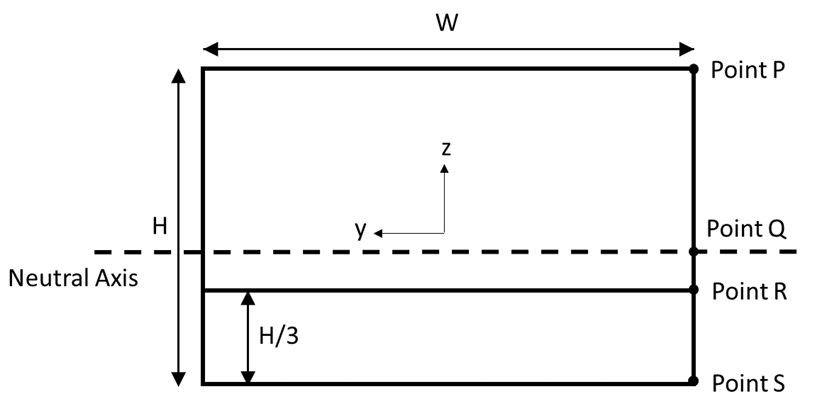
\includegraphics[width=0.4\columnwidth]{figs/fig-9.jpeg}
    \caption*{Fig-9:Midship section}
    \label{fig:9}
\end{figure}
\begin{enumerate}[leftmargin=2.5em, labelsep=0.5em, itemsep=0.5em]
    \item Magnitude of longitudinal bending stress is maximum at point P and magnitude of vertical shear stress is maximum at point Q.
    \item Magnitude of longitudinal bending stress is maximum at point S and magnitude of vertical shear stress is maximum at point R.
    \item Magnitude of longitudinal bending stress is maximum at point Q and magnitude of vertical shear stress is maximum at point S.
    \item Magnitude of longitudinal bending stress is maximum at point R and magnitude of vertical shear stress is maximum at point P.
\end{enumerate}
\end{enumerate}
\newpage
\vspace*{0.25cm}

\begin{enumerate}[itemsep=1em]
\setcounter{enumi}{26}
\item Consider a Planar Motion Mechanism (PMM) test of a ship model in a towing tank. The transverse motion of the model from the centerline of the tank is described by $y=a_0\cos({\omega t})$, where $\omega$ is the angular frequency. The carriage speed is 3 m/s, $\omega = \frac{\sqrt{3}}{2}$ rad/s and the maximum drift angle during the test is $30\degree$. The amplitude of oscillation $a_0$ lies between \underline{\hspace{2cm}}. 
\begin{multicols}{4}
\begin{enumerate}
    \item 0.2 m and 0.4 m
    \item 0.5 m and 0.7 m
    \item 1.0 m and 1.2 m
    \item 1.9 m and 2.1 m
\end{enumerate}    
\end{multicols}
\end{enumerate}

\begin{enumerate}[itemsep=1em]
\setcounter{enumi}{27}
\item Consider the function $f(x)=|x|-1$. Which of the following statements is/are true in the interval [-10,10]? 
\begin{enumerate}[leftmargin=2.5em, labelsep=0.5em, itemsep=0.5em]
    \item The function is differentiable in the domain. 
    \item The function is continuous in the domain.
    \item The function is not differentiable in the domain. 
    \item The function is not continuous in the domain. 
\end{enumerate}
\end{enumerate}

\begin{enumerate}[itemsep=1em]
\setcounter{enumi}{28}
\item For a freely floating body in water, which of the following degrees of freedom has/have inherent restoring force? 
\begin{multicols}{4}
\begin{enumerate}
    \item Sway
    \item Surge
    \item Heave
    \item Pitch
\end{enumerate}
\end{multicols}
\end{enumerate}

\begin{enumerate}[itemsep=1em]
\setcounter{enumi}{29}
\item Which of the following boiler arrangements will ensure that there is \textbf{NO} contamination of the primary feed system? 
\begin{enumerate}[leftmargin=2.5em, labelsep=0.5em, itemsep=0.5em]
    \item Steam-to-steam generator
    \item Double evaporation boiler
    \item Water tube boiler
    \item Fire tube boiler
\end{enumerate}
\end{enumerate}

\begin{enumerate}[itemsep=1em]
\setcounter{enumi}{30}
\item Which of the following components is/are \textbf{NOT} found in a two-stroke marine diesel engine? 
\begin{multicols}{4}
\begin{enumerate}
    \item Crankshaft 
    \item Piston
    \item Spark plug
    \item Air-inlet valve
\end{enumerate}
\end{multicols}
\end{enumerate}

\begin{enumerate}[itemsep=1em]
\setcounter{enumi}{31}
\item Choose the correct statement(s) from the following with respect to a ship generated Kelvin wave pattern in deep water. 
\newpage
\vspace*{0.25cm}
\begin{enumerate}[leftmargin=2.5em, labelsep=0.5em, itemsep=0.5em]
    \item A system of transverse waves and divergent waves are observed behind the ship.
    \item A system of transverse waves and divergent waves are observed in front of the ship.
    \item The waves are contained in a sector originating at the bow with a half angle of $9\degree 28'$.
    \item The amplitude of wave components decrease as they propagate. 
\end{enumerate}
\end{enumerate}

\begin{enumerate}[itemsep=1em]
\setcounter{enumi}{32}
\item A box contains 12 red and 8 blue balls. Two balls are drawn randomly from the box without replacement.\\
\\
The probability of drawing a pair of balls having the same color is \underline{\hspace{2cm}} (rounded off to three decimal places).
\end{enumerate}

\begin{enumerate}[itemsep=1em]
\setcounter{enumi}{33}
\item The dynamics of a 90 m long ship are governed by the non-dimensional Nomoto equation. The magnitude of Nomoto gain $|K'|=\frac{72}{35\pi}$ and that of Nomoto time constant $|T'|=\frac{288}{35\pi}$  \\
\\
The steady turning radius of the ship for a $35\degree$ turning circle maneuver is \underline{\hspace{2cm}} m (answer in integer). 
\end{enumerate}

\begin{enumerate}[itemsep=1em]
\setcounter{enumi}{34}
\item A ship of length 200 m has a beam of 25 m. She floats in seawater with an even keel draught of 5 m. The prismatic coefficient of the ship is 0.9; the mass displacement is 20500 tonne and the density of seawater is 1025 $kg/m^3$.\\
\\
The midship section coefficient is \underline{\hspace{2cm}} (rounded off to two decimal places). 
\end{enumerate}

\subsubsection{\underline{Q.36 \text{-} Q.65 Carry TWO marks Each}}
\setlength{\parskip}{1em}

\begin{enumerate}[itemsep=1em]
\setcounter{enumi}{35}
\item 
Consider $f(t)=\cos(at)$, where a is a real constant. The Laplace transform of $f(t)$ is \underline{\hspace{2cm}}.  
\begin{multicols}{4}
\begin{enumerate}
    \item $\frac{a}{s^2+a^2}$
    \item $\frac{s}{s^2+a^2}$
    \item $\frac{a}{s^2-a^2}$
    \item $\frac{s}{s^2-a^2}$
\end{enumerate}
\end{multicols}
\end{enumerate}

\begin{enumerate}[itemsep=1em]
\setcounter{enumi}{36}
\item A square shaped body is subjected to only direct tensile stresses $\sigma_x$ and $\sigma_y$ as shown in the figure. If $\sigma_x>\sigma_y$, then the value of normal stress ($\sigma_{\theta}$) and shear stress ($\tau_{\theta}$) 
respectively are \underline{\hspace{2cm}}.
\begin{figure}[H]
    \centering
    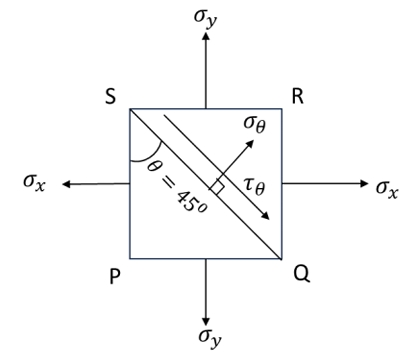
\includegraphics[width=0.4\columnwidth]{figs/fig-10.jpeg}
    \caption*{Fig-10:Square shaped body}
    \label{fig:10}
\end{figure}

\begin{multicols}{4}
\begin{enumerate}
    \item $\frac{\sigma_x-\sigma_y}{2}$ and $\frac{\sigma_x+\sigma_y}{2}$
    \item $\frac{\sigma_x+\sigma_y}{2}$ and $\frac{\sigma_x-\sigma_y}{2}$
    \item $\frac{\sigma_x+\sigma_y}{2}$ and $\frac{\sigma_x+\sigma_y}{2}$
    \item $\frac{\sigma_x-\sigma_y}{2}$ and $\frac{\sigma_x-\sigma_y}{2}$
\end{enumerate}    
\end{multicols}
\end{enumerate}



\begin{enumerate}[itemsep=1em]
\setcounter{enumi}{37}
\item The beam PQRS is subjected to a vertical point load of 10 kN at point S as shown in the figure. \\
\\
The magnitude of fixed end moment at P is \underline{\hspace{2cm}} kN-m. 
\begin{figure}[H]
    \centering
    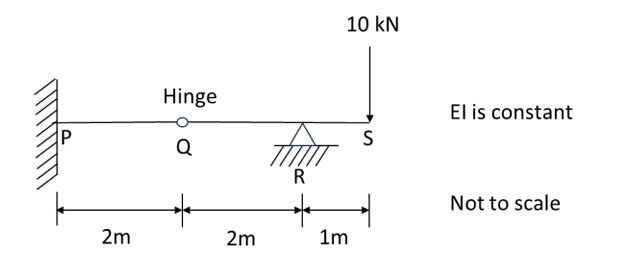
\includegraphics[width=0.4\columnwidth]{figs/fig-11.jpeg}
    \caption*{Fig-11:Beam PQRS}
    \label{fig:11}
\end{figure}
\begin{multicols}{4}
\begin{enumerate}
    \item 50
    \item 10
    \item 30
    \item 40
\end{enumerate}    
\end{multicols}
\end{enumerate}

\begin{enumerate}[itemsep=1em]
\setcounter{enumi}{38}
\item For a butt weld joint of two plates, which one of the following loading scenarios has the least permissible stress?  
\begin{multicols}{4}
\begin{enumerate}
    \item Tensile
    \item Bending
    \item Bearing
    \item Shear
\end{enumerate}
\end{multicols}
\end{enumerate}

\newpage
\vspace*{0.25cm}

\begin{enumerate}[itemsep=1em]
\setcounter{enumi}{39}
\item Match the non-dimensional numbers in Column 1 with the corresponding definitions in Column 2 
\begin{figure}[H]
    \centering
    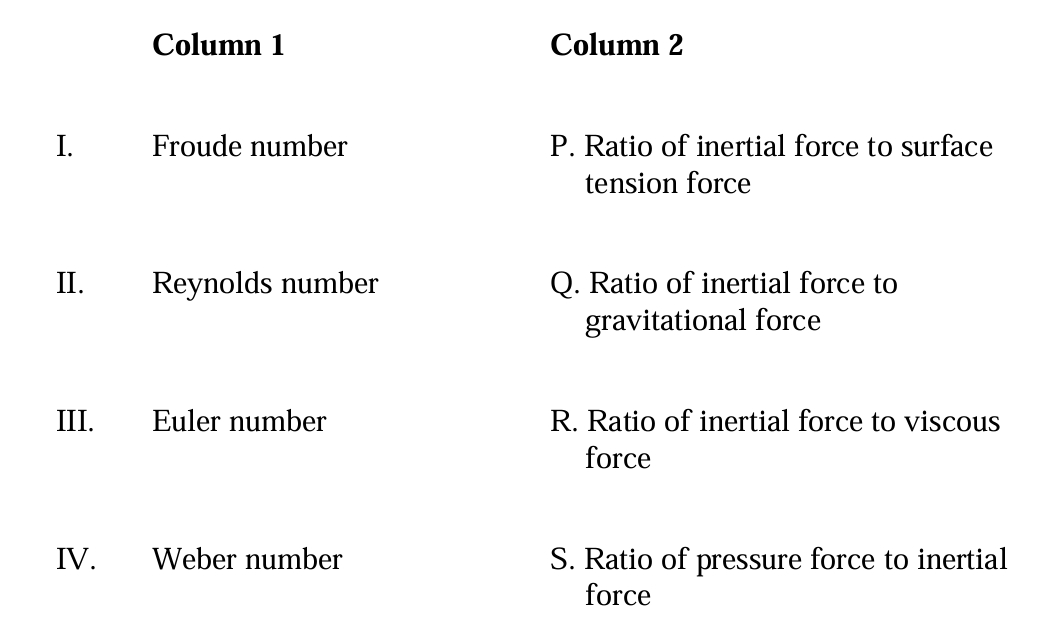
\includegraphics[width=0.6\columnwidth]{figs/fig-12.jpeg}
    \caption*{Column-match}
    \label{fig:12}
\end{figure}
\begin{enumerate}[leftmargin=2.5em, labelsep=0.5em, itemsep=0.5em]
    \item I-S;II-R;III-P;IV-Q
    \item I-Q;II-R;III-S;IV-P
    \item I-Q;II-R;III-P;IV-S
    \item I-S;II-Q;III-R;IV-P
\end{enumerate}
\end{enumerate}

\begin{enumerate}[itemsep=1em]
\setcounter{enumi}{40}
\item A closed system is undergoing a reversible process 1-P-2 from state 1 to 2, as shown in the figure, where X and Y are thermodynamic properties. An irreversible process 2-Q-1 brings the system back from 2 to 1. \\
\\
The net change in entropy of the system and surroundings during the above mentioned cycle are \underline{\hspace{2cm}} respectively.
\begin{figure}[H]
    \centering
    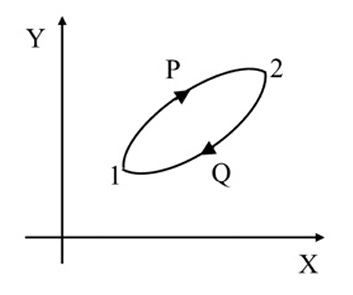
\includegraphics[width=0.4\columnwidth]{figs/fig-13.jpeg}
    \caption*{Fig-13:Graph of closed system undergoing thermodynamic process}
    \label{fig:13}
\end{figure}
\begin{enumerate}[leftmargin=2.5em, labelsep=0.5em, itemsep=0.5em]
    \item positive and negative
    \item negative and positive
    \item zero and negative
    \item zero and positive
\end{enumerate}
\end{enumerate}

\begin{enumerate}[itemsep=1em]
\setcounter{enumi}{41}
\item An ideal Brayton cycle (1-2-3-4) consisting of two isentropic and two isobaric processes is shown in the T-s plot, where T is the temperature and s is the specific entropy of the system. Which one of the following plots represents the corresponding actual cycle 1-2'-3-4' (denoted by dashed lines) between the same two pressures $p_1$ and $p_2$ ? 
\begin{figure}[H]
    \centering
    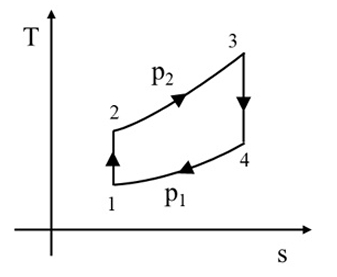
\includegraphics[width=0.2\columnwidth]{figs/fig-14.jpeg}
    \caption*{Fig-14:Ideal Brayton cycle}
    \label{fig:14}
\end{figure}
\begin{multicols}{4}
\begin{enumerate}
    \item \begin{minipage}[t]{0.2\textwidth}
    \vspace{0pt}
        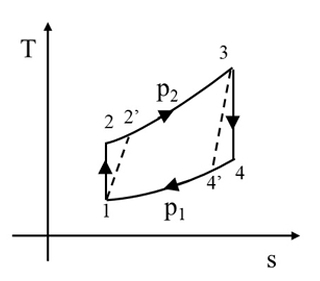
\includegraphics[width=\columnwidth]{figs/fig-15.jpeg}
        \label{fig:15}
    \end{minipage}
    \item \begin{minipage}[t]{0.2\textwidth}
    \vspace{0pt}
        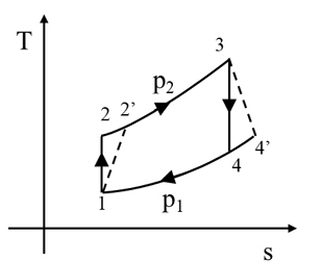
\includegraphics[width=\columnwidth]{figs/fig-16.jpeg}
        \label{fig:16}
    \end{minipage}
    \item \begin{minipage}[t]{0.2\textwidth}
    \vspace{0pt}
        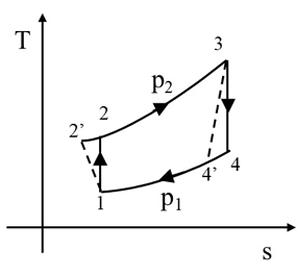
\includegraphics[width=\columnwidth]{figs/fig-17.jpeg}
        \label{fig:17}
    \end{minipage}
    \item \begin{minipage}[t]{0.2\textwidth}
    \vspace{0pt}
        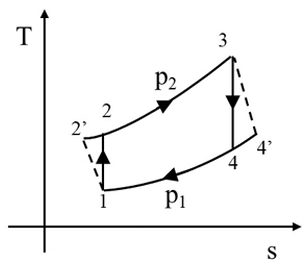
\includegraphics[width=\columnwidth]{figs/fig-18.jpeg}
    \label{fig:18}
    \end{minipage}
\end{enumerate}
\end{multicols}
\end{enumerate}

\begin{enumerate}[itemsep=1em]
\setcounter{enumi}{42}
\item Consider a rectangular barge of length $(L) = 100 \,\text{m}$, breadth $= 25 \,\text{m}$ and draught $= 10 \,\text{m}$.  
The barge has the following non-dimensional hydrodynamic derivatives with respect to a coordinate system whose origin is at the center of gravity:  
\\
$Y_{v}' = -1000 \times 10^{-5}, \quad N_{r}' = -800 \times 10^{-5}$,\\ 

$N_{v}' = -200 \times 10^{-5}, \quad Y_{r}' = 100 \times 10^{-5}$\\
\\
The stability criterion $C'$ is given by  \\

$C' = Y_{v}' \left( N_{r}' - m' x_{G}' \right) - \left( Y_{r}' - m' \right) N_{v}'$\\
\\
where $m' = \frac{m}{\tfrac{1}{2}\rho L^{3}}$, $m$ is the mass of the barge, $\rho$ is the density of seawater, and $x_{G}$ is the distance of the center of gravity from the origin. Which one of the following is correct regarding the controls-fixed straight-line stability?
\newpage
\vspace*{0.25cm}
\begin{enumerate}[leftmargin=2.5em, labelsep=0.5em, itemsep=0.5em]
    \item Unstable with $C^{'}=-1.8\times10^{-5}$
    \item Stable with $C^{'}=3.2\times10^{-5}$
    \item Stable with $C^{'}=-1.8\times10^{-5}$
    \item Unstable with $C^{'}=3.2\times10^{-5}$
\end{enumerate}
\end{enumerate}

\begin{enumerate}[itemsep=1em]
\setcounter{enumi}{43}
\item A ship has a propeller of 5 m pitch rotating at 120 rpm. The ship travels at 8 m/s and the wake fraction is 0.25. The apparent slip ratio and real slip ratio are \underline{\hspace{1cm}} respectively. 
\begin{multicols}{4}
\begin{enumerate}
    \item 0.20 and 0.40 
    \item 0.40 and 0.20 
    \item 0.20 and 0.25 
    \item 0.25 and 0.20 
\end{enumerate}
\end{multicols}
\end{enumerate}

\begin{enumerate}[itemsep=1em]
\setcounter{enumi}{44}
\item A ship of length 100 m and displacement 5000 tonne floats even-keel at 6.5 m in fresh water of density 1000 $kg/m^3$. The ship's hydrostatic properties are: \\
\\
MCT per cm is 10 tonne-m, 
TPC in seawater is 6.25,  
LCB is 2 m forward of amidship, 
LCF is 2 m forward of amidship.\\
\\
The ship has moved to seawater of density 1025 $kg/m^3$ without change in the 
displacement. The new forward and aft draughts are \underline{\hspace{1cm}} respectively.
\begin{enumerate}[leftmargin=2.5em, labelsep=0.5em, itemsep=0.5em]
    \item 6.04 m and 6.54 m 
    \item 6.30 m and 6.64 m 
    \item 6.64 m and 6.30 m 
    \item 6.30 m and 6.30 m 
\end{enumerate}
\end{enumerate}

\begin{enumerate}[itemsep=1em]
\setcounter{enumi}{45}
\item Consider a case where the load $Q$ for a ship structure has only statistical uncertainties. The probability density function of the load $p_Q(x)$ is shown in the figure. The characteristic limit value of the load ($Q_{L_c}$) is 1.5 and factor of safety is 1. Which of the following probability of exceedance value(s) of the load will lead to a safe design? 
\begin{figure}[H]
    \centering
    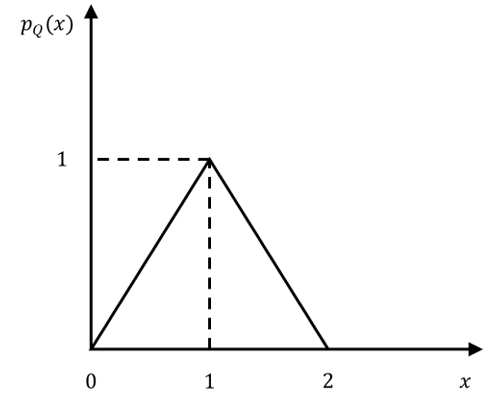
\includegraphics[width=0.3\columnwidth]{figs/fig-19.jpeg}
    \caption*{Fig-19}
    \label{fig:19}
\end{figure}
\newpage
\vspace*{0.25cm}
\begin{multicols}{4}
\begin{enumerate}
    \item 0.05
    \item 0.10
    \item 0.15
    \item 0.20
\end{enumerate}
\end{multicols}
\end{enumerate}

\begin{enumerate}[itemsep=1em]
\setcounter{enumi}{46}
    \item The value of $\int_1^3dy\int_2^5x^2y\,dx$ is \underline{\hspace{2cm}} (answer in integer).
\end{enumerate}

\begin{enumerate}[itemsep=1em]
\setcounter{enumi}{47}
\item Let $M=\myvec{1&&0\\0&&2}$ and $K=\myvec{2&&-1\\-1&&1}$  satisfy the eigenvalue problem given by $[M-\alpha K]\varphi=0$.\\
The lowest eigenvalue $\alpha$ is \underline{\hspace{1cm}} (rounded off to two decimal places). 
\end{enumerate}

\begin{enumerate}[itemsep=1em]
\setcounter{enumi}{48}
\item The gradient of $y=3x^2\sin(2x)$ at (0.2, 1) is \underline{\hspace{1cm}}(rounded off to three decimal places). 
\end{enumerate}

\begin{enumerate}[itemsep=1em]
\setcounter{enumi}{49}
\item A simply supported solid beam is subjected to a vertical point load of 10 N at the middle. The length of the beam is 4 m, and the cross section is $0.5 \,m \times 0.5 \,m$.\\  
The magnitude of maximum tensile stress in the beam is \underline{\hspace{1cm}} $N/m^2$ (answer in integer). 
\end{enumerate}

\begin{enumerate}[itemsep=1em]
\setcounter{enumi}{50}
\item The displacement field of a body is given by $\vec{u}=yx\,\hat{i} + yz\,\hat{j} + (z+x^2)\,\hat{k}$. The shear strain $\gamma_{xy}$ at (2, 1, 5) is \underline{\hspace{2cm}}(answer in integer). 
\end{enumerate}

\begin{enumerate}[itemsep=1em]
\setcounter{enumi}{51}
\item A freely-floating rectangular barge of length 200 m is divided into five equal compartments. In light-weight condition, the weight and buoyancy are uniformly distributed along the length of the barge. Assume g = 9.81 $m/s^2$. \\
If 500 tonne of liquid cargo is added to each of the two end compartments as shown in the figure, then the maximum bending moment is \underline{\hspace{2cm}} MN-m (rounded off to two decimal places). 
\begin{figure}[H]
    \centering
    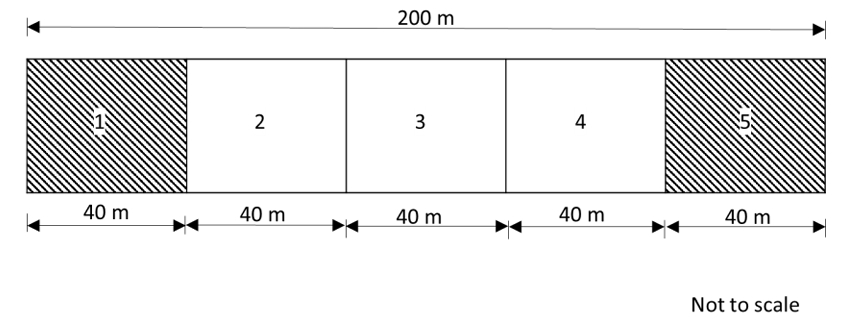
\includegraphics[width=0.4\columnwidth]{figs/fig-20.jpeg}
    \caption*{Fig-20:Free-floating rectangular barge}
    \label{fig:20}
\end{figure}
\end{enumerate}

\begin{enumerate}[itemsep=1em]
\setcounter{enumi}{52}
\item The stream function of a two-dimensional flow field is given as  
$\psi=2xy+2y+2x$. The coordinates of two points P and Q in the flow field are 
(1, 2) and (2, 5) respectively. \\
The magnitude of flow discharge between the streamlines passing through P and Q is \underline{\hspace{2cm}}(answer in integer). 
\end{enumerate}

\begin{enumerate}[itemsep=1em]
\setcounter{enumi}{53}
\item A tank with a constant water level of 4 m above the centreline of an opening of diameter 100 mm is shown in the figure. Neglect all losses and assume   $g = 9.81 m/s^2$. \\ 
The discharge through the opening is \underline{\hspace{2cm}} litre/s (answer in integer).  
\newpage
\vspace*{0.25cm}
\begin{figure}[H]
    \centering
    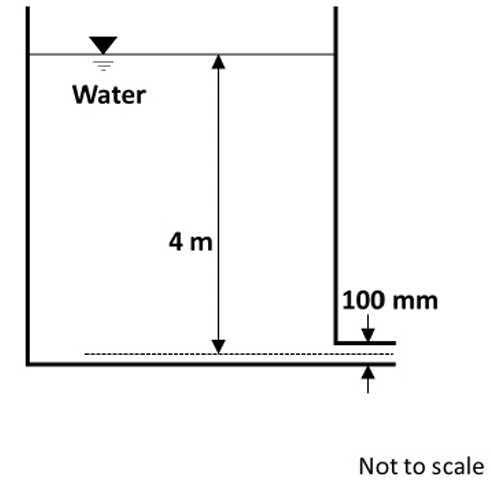
\includegraphics[width=0.4\columnwidth]{figs/fig-21.jpeg}
    \caption*{Fig-21:water tank}
    \label{fig:21}
\end{figure}
\end{enumerate}

\begin{enumerate}[itemsep=1em]
\setcounter{enumi}{54}
\item Air flows with a velocity of 2 m/s over a flat stationary surface parallel to its length of 0.5 m. Kinematic viscosity of air $v$ is $1.5 \times 10^{-5} \,m^2/s$.  \\
Using Blasius solution, the boundary layer thickness at the trailing edge of the surface is \underline{\hspace{2cm}} mm (rounded off to two decimal places). 
\end{enumerate}

\begin{enumerate}[itemsep=1em]
\setcounter{enumi}{55}
\item A negligibly thin horizontal plate PQ has a length 3 m and width 1 m. It is being pulled along its length at a speed of 1 m/s in between two static parallel plates as shown in the figure. The gap of 6 cm between the plates is filled with a Newtonian fluid of dynamic viscosity $\mu = 0.2\; N-s/m^2$. The thin plate is located at 3 cm from the top surface. The velocity distribution between the thin plate and the static plates is linear.  The steady force required to pull the plate is \underline{\hspace{2cm}}N (answer in integer). 
\begin{figure}[H]
    \centering
    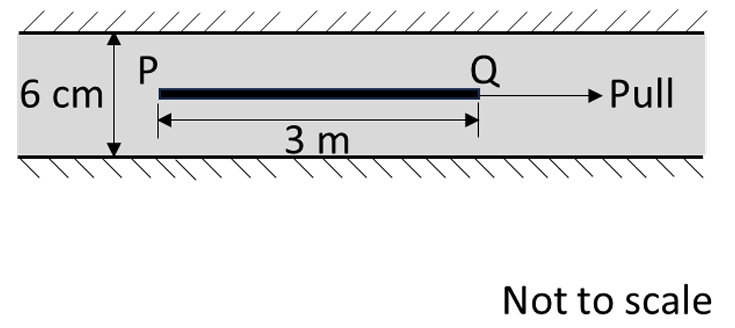
\includegraphics[width=0.4\columnwidth]{figs/fig-22.jpeg}
    \caption*{Fig-22}
    \label{fig:22}
\end{figure}
\end{enumerate}

\begin{enumerate}[itemsep=1em]
\setcounter{enumi}{56}
\item Water of density $\rho = 1000 \,kg/m^3$ flows with a velocity V = 50 m/s through a $180\degree$ curved tube of uniform cross-section as shown in the figure. If the flow rate is 0.06 $m^3/s$, the magnitude of reaction force $F_x$ required to keep it stationary is \underline{\hspace{2cm}} kN (rounded off to one decimal place).
\newpage
\vspace*{0.25cm}
\begin{figure}[H]
    \centering
    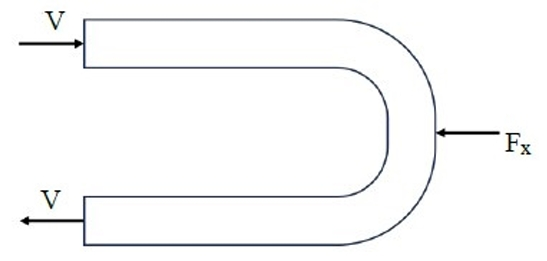
\includegraphics[width=0.4\columnwidth]{figs/fig-23.jpeg}
    \caption*{Fig-23:Curved tube of uniform cross section}
    \label{fig:23}
\end{figure}
\end{enumerate}

\begin{enumerate}[itemsep=1em]
\setcounter{enumi}{57}
\item An ocean wave is propagating from deep to shallow water. The wave is approaching the coast at $45\degree$ counterclockwise from the shore normal with an initial phase speed of 12.5 m/s. After entering the shallow water, the wave direction becomes $30\degree$ counterclockwise from the shore normal. \\
The phase speed of the wave at the shallow water is \underline{\hspace{2cm}} m/s (rounded off to one decimal place). 
\end{enumerate}

\begin{enumerate}[itemsep=1em]
\setcounter{enumi}{58}
\item Consider the psychrometric process denoted by the straight line from state 1 to 2 in the figure. The specific humidity, Dry Bulb Temperature (DBT) and Wet Bulb Temperature (WBT) at the two states are shown in the table. The latent heat of vaporization of water (hfg) is 2440 kJ/kg. \\  
If the flow rate of air is 1 kg/s, the rate of heat transfer from the air is \underline{\hspace{2cm}} kW (rounded off to two decimal places). 
\begin{figure}[H]
    \centering
    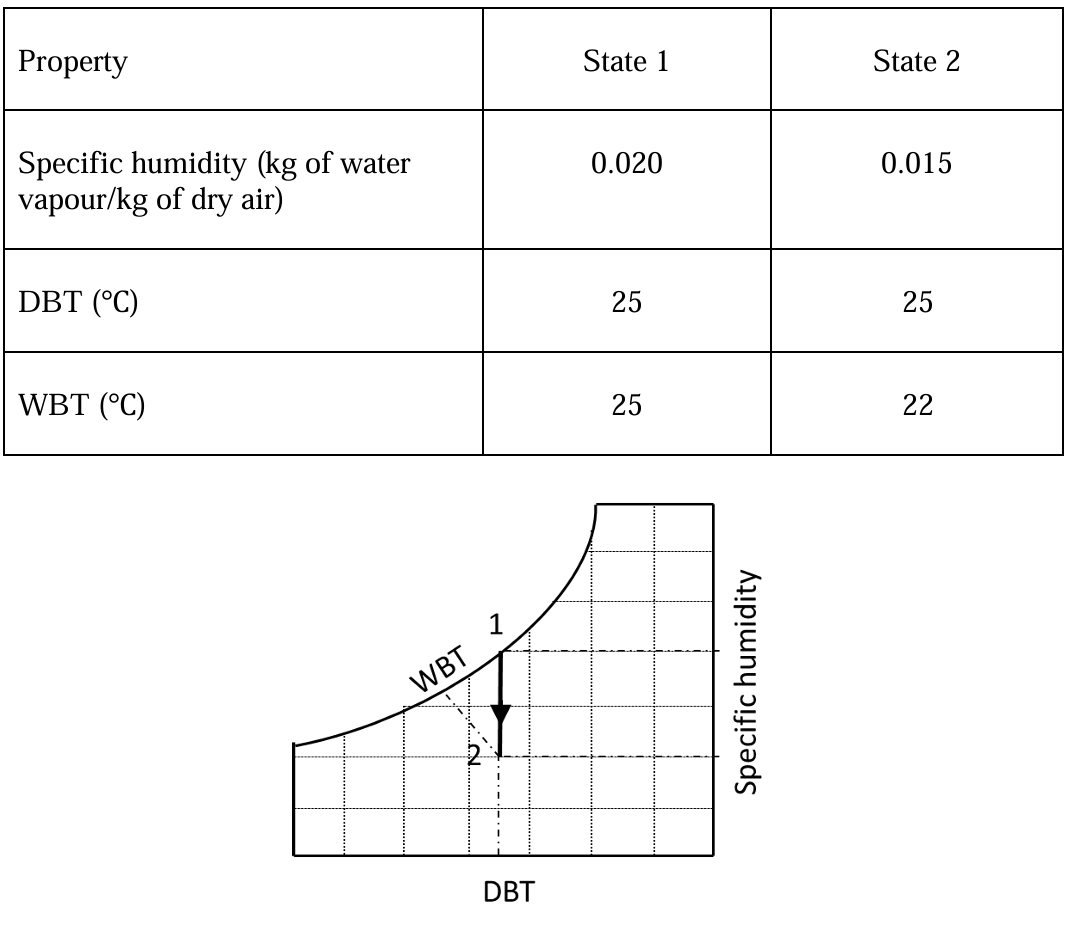
\includegraphics[width=0.6\columnwidth]{figs/fig-24.jpeg}
    \caption*{Fig-24:Psychometric process}
    \label{fig:24}
\end{figure}
\end{enumerate}
\newpage
\vspace*{0.25cm}
\begin{enumerate}[itemsep=1em]
\setcounter{enumi}{59}
\item Consider a weightless, frictionless piston with a 2 kg mass placed on it as shown in the figure. At equilibrium in position 1, the cylinder contains 0.1 kg of air. The piston cross-sectional area is 0.01 $m^2$. The ambient pressure in the surroundings outside the piston-cylinder arrangement is 0 bar (absolute). When the mass above the piston is removed instantaneously, it moves up and hits the stop at position 2 which is 0.1 m above the initial position. Assuming g = 9.81 $m/s^2$,the thermodynamic work done by the system during this process is \underline{\hspace{2cm}} J (answer in integer). 
\begin{figure}[H]
    \centering
    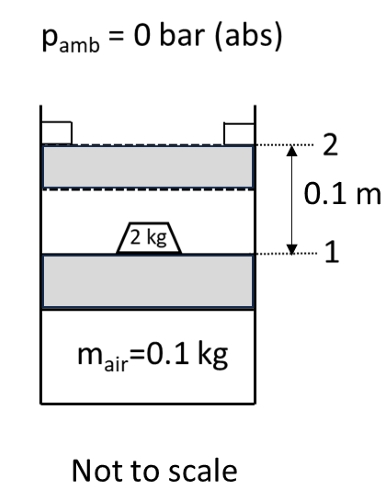
\includegraphics[width=0.3\columnwidth]{figs/fig-25.jpeg}
    \caption*{Fig-25:Weightless, frictionless piston}
    \label{fig:25}
\end{figure}
\end{enumerate}

\begin{enumerate}[itemsep=1em]
\setcounter{enumi}{60}
\item A two-stroke four-cylinder large marine diesel engine has a cylinder bore of 600 mm and stroke length of 2400 mm. The brake thermal efficiency $(\eta_{bth})$ is 45\% and fuel consumption rate ($\dot{m}_f$) is 0.265 kg/s at an engine speed (N) of 100 rpm.Assuming the calorific value of fuel is 42 MJ/kg, the brake mean effective pressure (bmep) is \underline{\hspace{2cm}} bar (rounded off to one decimal place).
\end{enumerate}

\begin{enumerate}[itemsep=1em]
\setcounter{enumi}{61}
\item A multi-cell midship section of a ship with B = 40 m and D = 20 m is shown in the figure. The shear-flows are given as $q_1=q_2=q_3=0.9376$ MN/m.
he applied twisting moment on the midship section is \underline{\hspace{2cm}} MN-m (rounded off to two decimal places).
\newpage
\vspace*{0.25cm}
\begin{figure}[H]
    \centering
    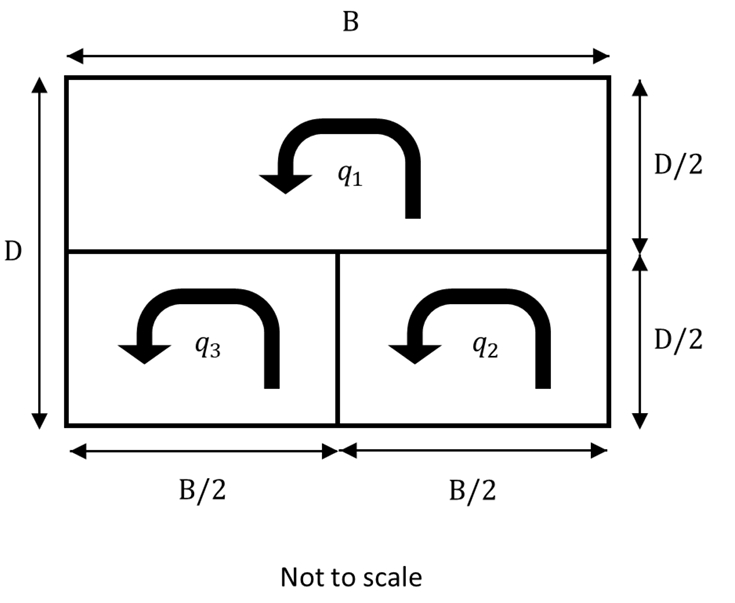
\includegraphics[width=0.3\columnwidth]{figs/fig-26.jpeg}
    \caption*{Fig-26:Multi-cell midship section}
    \label{fig:26}
\end{figure}
\end{enumerate}

\begin{enumerate}[itemsep=1em]
\setcounter{enumi}{62}
\item A ship of 3300 tonne displacement is undergoing an inclining experiment in seawater of density 1025 $kg/m^3$. A mass of 6 tonne is displaced transversely by 12 m as shown in the figure. This results in 0.12 m deflection of a 11 m long pendulum suspended from the centerline. The transverse metacenter of the ship is located at 7.25 m above the keel.The distance of the center of gravity from the keel is \underline{\hspace{2cm}} m (rounded off to two decimal places).
\begin{figure}[H]
    \centering
    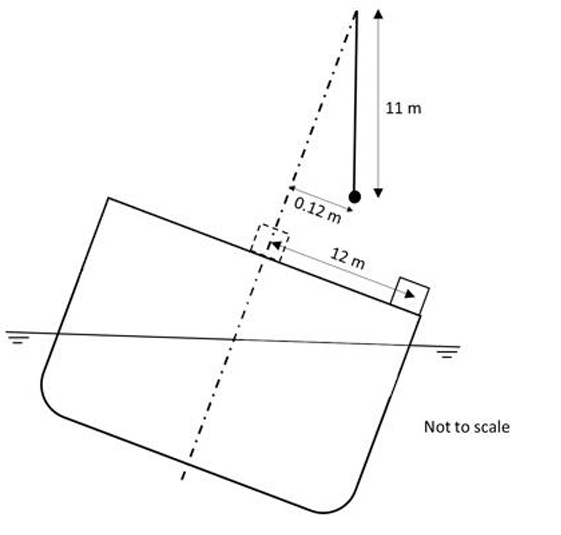
\includegraphics[width=0.3\columnwidth]{figs/fig-27.jpeg}
    \caption*{Fig-27:Figure of inclined ship}
    \label{fig:27}
\end{figure}
\end{enumerate}

\begin{enumerate}[itemsep=1em]
\setcounter{enumi}{63}
\item A ship moving at a steady forward speed of 10 m/s experiences a total resistance of 140 kN. The Quasi Propulsive Coefficient (QPC) is 0.70; the propeller shaft losses are 5\% and the mechanical efficiency of the main engine is 80\%. The indicated power of the main engine is \underline{\hspace{2cm}} kW (rounded off to two decimal places). 
\end{enumerate}

\begin{enumerate}[itemsep=1em]
\setcounter{enumi}{64}
\item A single degree of freedom system is undergoing free oscillation. The natural frequency and damping ratio of the system are 1 rad/sec and 0.01 respectively. The reduction in peak amplitude over three cycles is \underline{\hspace{2cm}} \% (rounded off to one decimal place).
\end{enumerate}


\end{document}